%%13:6:24 25/1/2017 -VieTeX creates E:\tex\book-mau\mau-soanthao-tracnghiem\cauhoi-nguyenthiminhkhai.tex
\begin{question}%1
Hàm số $y=x.e^x$ tăng trong khoảng
\datcot
\bonpa
{\dung{$\left(-1; +\infty\right)$.}}
{\sai{$\left(-2; +\infty\right)$.}}
{\sai{$\left(-\infty; -1\right)$.}}
{\sai {$\left(-\infty; -2\right)$.}}
\end{question}

\begin{question}%2
Giá trị $m$ để hàm số $y=2x^3-(m+5)x^2+6mx+3$ đạt cực tiểu tại $x=2$ là
\datcot
\bonpa
{\dung{$-2$.}}
{\sai{$-1$.}}
{\sai{$2$.}}
{\sai {$1$.}}
\end{question}

\begin{question}%3
Phương trình tiếp tuyến với $(C): y=\dfrac{x+2}{2x-3}$ tại giao điểm của $(C)$ với trục hoành là
\datcot
\bonpa
{\sai{$y=\dfrac{1}{7}(x-2)$.}}
{\dung{$y=-\dfrac{1}{7}(x+2)$.}}
{\sai{$y=-\dfrac{1}{7}(x-2)$.}}
{\sai {$y=-\dfrac{x}{7}$.}}
\end{question}

\begin{question}%4
Số giao điểm của đường cong $(C): y=\dfrac{3x^2}{x+2}$ và đường thẳng $(D): y=2-x$ là
\datcot
\bonpa
{\dung{$2$.}}
{\sai{$0$.}}
{\sai{$1$.}}
{\sai {$3$.}}
\end{question}

\begin{question}%5
Giá trị lớn nhất và giá trị nhỏ nhất của hàm số $y=x^3-3x^2-9x+2$ trên đoạn $\left[-2; 2\right]$ lần lượt là:
\datcot
\bonpa
{\dung{7 và -20.}}
{\sai{7 và 2.}}
{\sai{7 và $-1$.}}
{\sai{7 và 0.}}
\end{question}

\begin{question}%6
Chọn phát biểu \textbf{SAI}
\datcot[4]
\bonpa
{\dung{Đồ thị hàm số $y=\dfrac{x}{x^2+2}$ chỉ có 1 tiệm cận đứng.}}
{\sai{Đồ thị hàm số $y=x^4-2x^2+1$ không có tiệm cận nào.}}
{\sai{Đồ thị hàm số $y=\dfrac{x}{x+2}$ có 2 tiệm cận.}}
{\sai{Đồ thị hàm số $y=\dfrac{x}{x^2+2}$ chỉ có 1 tiệm cận ngang.}}
\end{question}

\begin{question}%7
Đồ thị dưới đây là của hàm số nào?
\begin{center}
\definecolor{ffqqqq}{rgb}{1.,0.,0.}
\begin{tikzpicture}[line cap=round,line join=round,>=triangle 45,x=1.0cm,y=1.0cm]
\draw[->,color=black] (-2.6,0.) -- (3.18,0.);
\foreach \x in {-2.,-1.,1.,2.,3.}
\draw[shift={(\x,0)},color=black] (0pt,2pt) -- (0pt,-2pt) node[below] {\footnotesize $\x$};
\draw[->,color=black] (0.,-1.8) -- (0.,3.98);
\foreach \y in {-1.,1.,2.,3.}
\draw[shift={(0,\y)},color=black] (2pt,0pt) -- (-2pt,0pt) node[left] {\footnotesize $\y$};
\draw[color=black] (0pt,-10pt) node[right] {\footnotesize $0$};
\clip(-2.6,-1.8) rectangle (3.18,3.98);
\draw[line width=1.2pt,color=ffqqqq,smooth,samples=100,domain=-2.4:3.0] plot(\x,{(\x)^(4.0)-2.0*(\x)^(2.0)});
\end{tikzpicture}
\end{center}
\datcot
\bonpa
{\dung{$y=x^4-2x^2$.}}
{\sai{$y=-x^3+3x^2$.}}
{\sai{$y=x^4-2x^2+2$.}}
{\sai{$y=x^4+2x^2$.}}
\end{question}

\begin{question}%8
Giá trị biểu thức $L=\dfrac{\log_2 240}{\log_{3.75} 2}-\dfrac{\log_2 15}{\log_{60} 2}+\log_2 1$ là
\vspace{0.3cm}
\datcot
\bonpa
{\dung{$-8$.}}
{\sai{$8$.}}
{\sai{$0$.}}
{\sai{$1$.}}
\end{question}

\begin{question}%9
Cho $0< a< b$ và $x>0$. Chọn kết quả \textbf{Đúng}
\datcot
\bonpa
{\dung{$a^x< b^x$.}}
{\sai{$a^x > b^x$.}}
{\sai{$a^x= b^x$.}}
{\sai{$a^x \geq b^x$.}}
\end{question}

\begin{question}%10
Phương trình $2^{2x+1}=\left(\dfrac{1}{2}\right)^{2x+3}$
\datcot
\bonpa
{\dung{$x=-1$.}}
{\sai{$x=0$.}}
{\sai{$x=1$.}}
{\sai{$x=3$.}}
\end{question}

\begin{question}%11
Tập nghiệm của bất phương trình $\dfrac{1}{9}.3^{2x}>1$ là:
\datcot
\bonpa
{\sai{$\left[1; +\infty\right)$.}}
{\dung{$\left(1; +\infty\right)$.}}
{\sai{$\left(0; +\infty\right)$.}}
{\sai{$\left[0; +\infty\right)$.}}
\end{question}

\begin{question}%12
Phương trình $\log_2 x+\log_2\left(x^2\right)=\log_2\left(4x\right)$ có tập nghiệm là:
\datcot
\bonpa
{\sai{$\left\lbrace 0; -2; 2\right\rbrace$.}}
{\sai{$\left\lbrace 0; 2\right\rbrace$.}}
{\sai{$\left\lbrace -2; 2\right\rbrace$.}}
{\dung{$\left\lbrace 2\right\rbrace$.}}
\end{question}

\begin{question}%%13
Bất phương trình $\log_2\left(1+3^x\right)+\log_{\left(1+3^x\right)}2-2>0$ có nghiệm là:
\datcot
\bonpa
{\sai{$x>0$.}}
{\sai{$x<0$.}}
{\dung{$x \neq 0$.}}
{\sai{$x$ tùy ý.}}
\end{question}

\begin{question}%%14
Hàm số $y=\dfrac{2x-m^2}{x-2}$ đồng biến trong từng khoảng xác định khi và chỉ khi
\datcot
\bonpa
{\dung{$m<-2 \vee m>2$.}}
{\sai{$m\leq -2 \vee m\geq 2$.}}
{\sai{$m\leq -2$.}}
{\sai{$m\geq 2$.}}
\end{question}

\begin{question}%%15
Giá trị $m<0$ sao cho đường thẳng $y=m$ và đồ thị hàm số $y=\dfrac{x^3}{3}-x^2+1$ có 2 điểm chung phân biệt là:
\datcot
\bonpa
{\sai{$m=-1$.}}
{\sai{$m=-\dfrac{1}{2}$.}}
{\dung{$m=-\dfrac{1}{3}$.}}
{\sai{$m=-\dfrac{1}{4}$.}}
\end{question}

\begin{question}%%16
Cho hàm số $y=\dfrac{4x-2}{x-3}$ có đồ thị $(C)$. Có bao nhiêu tiếp tuyến của $(C)$ đi qua điểm $I(3;4)$?
\vspace{0.2cm}
\datcot
\bonpa
{\sai{2.}}
{\dung{0.}}
{\sai{1.}}
{\sai{3.}}
\end{question}

\begin{question}%%17
Đồ thị hàm số $y=-2x^3+(m+3)x^2+5$ có duy nhất 1 điểm cực trị khi và chỉ khi
\vspace{0.2cm}
\datcot
\bonpa
{\sai{$m=0$.}}
{\dung{$m \leq -3$.}}
{\sai{$m<-3$.}}
{\sai{$m>-3$.}}
\end{question}

\begin{question}%%18
Cho hàm số $y=\dfrac{x+2}{x-1}$ có đồ thị $(C)$. Chọn kết quả \textbf{SAI}:
\vspace{0.2cm}
\datcot[4]
\bonpa
{\dung{Hàm số nghịch biến trên khoảng $\left(0; +\infty\right)$.}}
{\sai{$(C)$ có 1 tiệm cận ngang.}}
{\sai{$(C)$ có tâm đối xứng là $I(1; 1)$.}}
{\sai{$(C)$ không có điểm chung với đường thẳng $(D): y=1$.}}
\end{question}

\begin{question}%%19
Gọi $x_1, x_2$ là 2 nghiệm của phương trình $5^{2x+1}-8.5^x+1=0$. Khi đó:
\vspace{0.2cm}
\datcot
\bonpa
{\sai{$x_1 + x_2=1$.}}
{\sai{$x_1 + x_2=-2$.}}
{\sai{$x_1+ x_2=2$.}}
{\dung{$x_1+x_2=-1$.}}
\end{question}

\begin{question}%%20
Nếu $a^{\frac{3}{4}}> a^{\frac{4}{5}}$ và $\log_b \dfrac{1}{2}<\log_b \dfrac{2}{2}$ thì ta có:
\vspace{0.2cm}
\datcot
\bonpa
{\sai{$0<a<b<1$.}}
{\sai{$0<b<a<1$.}}
{\dung{$0<a<1<b$.}}
{\sai{$1<a<b$.}}
\end{question}

\begin{question}%%21
Cho $f(x)=\ln\left|\cos 3x\right|$. Giá trị $f'\left(\dfrac{\pi}{12}\right)$:
\vspace{0.2cm}
\datcot
\bonpa
{\dung{$-3$.}}
{\sai{$3$.}}
{\sai{$2$.}}
{\sai{$1$.}}
\end{question}

\begin{question}%%22
Phương trình $2^x=5^{x+1}$ có nghiệm là
\vspace{0.2cm}
\datcot
\bonpa
{\sai{$x=\log_2 5$.}}
{\dung{$\log_{\frac{2}{5}} 5$.}}
{\sai{$x=\log_5 2$.}}
{\sai{$x=0$.}}
\end{question}

\begin{question}%%23
Tập nghiệm của phương trình: $\dfrac{1}{2}\lg\left(152+x^2\right)=\lg\left(x+2\right)$
\vspace{0.2cm}
\datcot
\bonpa
{\sai{$\left\lbrace 36\right\rbrace$.}}
{\dung{$\left\lbrace 37\right\rbrace$.}}
{\sai{$\left\lbrace 38\right\rbrace$.}}
{\sai{$\left\lbrace 39\right\rbrace$.}}
\end{question}

\begin{question}%%24
Tập xác định của hàm số: $y=\sqrt{\ln\left(\dfrac{x^2-3}{2x}\right)}$
\vspace{0.2cm}
\datcot
\bonpa
{\sai{$\left(-1; 0\right) \cup \left(3; +\infty\right)$.}}
{\sai{$\left[-1; 0\right) \cup \left(3; +\infty\right)$.}}
{\dung{$\left[-1; 0\right) \cup \left[3; +\infty\right)$.}}
{\sai{$\left[-1; 0\right] \cup \left[3; +\infty\right)$.}}
\end{question}

\begin{question}%%25
Hàm số $y=\log_2\left[\log_5\left(\left(m-2\right)x^2+2(m-3)+m\right)\right]$ có tập xác định là $\mathbb{R}$ khi giá trị $m$ thỏa
\vspace{0.2cm}
\datcot
\bonpa
{\dung{$m>\dfrac{7}{3}$.}}
{\sai{$m \geq \dfrac{7}{3}$.}}
{\sai{$m<\dfrac{7}{3}$.}}
{\sai{$m \leq \dfrac{7}{3}$.}}
\end{question}

\begin{question}%%26
Với giá trị nào của $k$ thì đường thẳng $y=kx+1$ cắt đồ thị hàm số $y=x^3+x+1$ tại 3 điểm phân biệt.
\vspace{0.2cm}
\datcot
\bonpa
{\sai{$k>0$.}}
{\dung{$k>1$.}}
{\sai{$k<1$.}}
{\sai{$k\leq 1$.}}
\end{question}

\begin{question}%%27
Cho hàm số $f$ có đạo hàm $f'(x)=x^4(x-1)(2-x)^3(x-4)^4$. Số cực trị của hàm số $f$ là:
\vspace{0.2cm}
\datcot
\bonpa
{\sai{$4$.}}
{\sai{$3$.}}
{\dung{$2$.}}
{\sai{$1$.}}
\end{question}

\begin{question}%%28
Số tiếp tuyến của đồ thị $(C): y=x^3-3x^2+2$ đi qua điểm $M(1; 0)$ là
\vspace{0.2cm}
\datcot
\bonpa
{\dung{$1$.}}
{\sai{$2$.}}
{\sai{$3$.}}
{\sai{$4$.}}
\end{question}

\begin{question}%%29
Giá trị nhỏ nhất của hàm số $y=2^{x-1}+2^{3-x}$ bằng
\vspace{0.2cm}
\datcot
\bonpa
{\sai{$1$.}}
{\sai{$2$.}}
{\sai{$3$.}}
{\dung{$4$.}}
\end{question}

\begin{question}%%30
Cho biết đồ thị hàm số $y=\dfrac{x+2}{x-1}$ cắt đường thẳng $d: y=x+m$ tại hai điểm phân biệt $A, B$ sao cho trung điểm $I$ của đoạn $AB$ nằm trên trục hoành. Khi đó:
\vspace{0.2cm}
\datcot
\bonpa
{\sai{$m=1$.}}
{\dung{$m=-2$.}}
{\sai{$m=3$.}}
{\sai{$m=4$.}}
\end{question}

\begin{question}%%31
Khối chóp $n-$ giác có tất cả bao nhiêu cạnh?
\vspace{0.2cm}
\datcot
\bonpa
{\sai{$n$.}}
{\sai{$n+1$.}}
{\sai{$n+2$.}}
{\dung{$2n$.}}
\end{question}

\begin{question}%%32
Khối lập phương là khối đa diện đều thuộc loại
\vspace{0.2cm}
\datcot
\bonpa
{\dung{$\left\lbrace 4; 3\right\rbrace$.}}
{\sai{$\left\lbrace 5; 3\right\rbrace$.}}
{\sai{$\left\lbrace 3; 4\right\rbrace$.}}
{\sai{$\left\lbrace 3; 3\right\rbrace$.}}
\end{question}

\begin{question}%%33
Nếu một hình chóp đều có chiều cao và cạnh đáy cùng tăng lên 5 lần thì thể tích của nó tăng lên:
\vspace{0.2cm}
\datcot
\bonpa
{\sai{5 lần.}}
{\sai{25 lần.}}
{\dung{125 lần.}}
{\sai{10 lần.}}
\end{question}

\begin{question}%%34
Cho hình chóp $S.ABCD$ có đáy $ABCD$ là hình vuông cạnh $a$, $SA \bot (ABCD)$, $SA= a$. Góc giữa đường thẳng $SB$ và mặt phẳng $(ABCD)$ bằng:
\vspace{0.2cm}
\datcot
\bonpa
{\sai{$30^0$.}}
{\dung{$45^0$.}}
{\sai{$60^0$.}}
{\sai{$90^0$.}}
\end{question}

\begin{question}%%35
Khối chóp tam giác đều có cạnh đáy bằng $a$, cạnh bên hợp với mặt đáy góc $30^0$. Thể tích khối chóp bằng
\vspace{0.2cm}
\datcot
\bonpa
{\dung{$\dfrac{a^3\sqrt{3}}{36}$.}}
{\sai{$\dfrac{a^3\sqrt{3}}{6}$.}}
{\sai{$a^3\sqrt{3}$.}}
{\sai{$\dfrac{a^3\sqrt{3}}{3}$.}}
\end{question}

\begin{question}%%36
Cho hình chóp $O.ABC$ có $OA$, $OB$, $OC$ đôi một vuông góc; $OA=3a$, $OB=4a$, $OC=5a$. Diện tích mặt cầu ngoại tiếp hình chóp bằng
\vspace{0.2cm}
\datcot
\bonpa
{\sai{$20\pi a^2$.}}
{\sai{$30\pi a^2$.}}
{\dung{$50 \pi a^2$.}}
{\sai{$80\pi a^2$.}}
\end{question}

\begin{question}%%37
Cho hình trụ có diện tích thiết diện qua trục là 25. Diện tích xung quanh của hình trụ bằng
\vspace{0.2cm}
\datcot
\bonpa
{\sai{$250\pi$.}}
{\dung{$25\pi$.}}
{\sai{$50\pi$.}}
{\sai{$50$.}}
\end{question}

\begin{question}%%38
Một hình nón có bán kính bằng $R$ và diện tích xung quanh bằng $\dfrac{5\pi R^2}{3}$. Khi đó diện tích của khối nón bằng
\vspace{0.2cm}
\datcot
\bonpa
{\dung{$\dfrac{4\pi R^3}{9}$.}}
{\sai{$\dfrac{4\pi R^2}{9}$.}}
{\sai{$\dfrac{4\pi R}{9}$.}}
{\sai{$\dfrac{2\pi R^3}{9}$.}}
\end{question}

\begin{question}%%39
Khối chóp $S.ABCD$ có $A, B, C, D$ cố định và $S$ chạy trên 1 đường thẳng song song với $AC$. Khi đó thể tích khối chóp $S.ABCD$ sẽ:
\vspace{0.2cm}
\datcot
\bonpa
{\dung{Giữ nguyên.}}
{\sai{Tăng gấp đôi.}}
{\sai{Giảm phân nửa.}}
{\sai{Tăng gấp bốn.}}
\end{question}

\begin{question}%%40
Khối lăng trụ đều $ABC.A'B'C'$ có $AB=2a, AA'=4a$. Thể tích $ABC.A'B'C'$ có giá trị bằng
\vspace{0.2cm}
\datcot
\bonpa
{\sai{$a^3\sqrt{3}$.}}
{\dung{$4a^3\sqrt{3}$.}}
{\sai{$2a^3\sqrt{3}$.}}
{\sai{$3a^3\sqrt{3}$.}}
\end{question}

\begin{question} %%41
Khối hộp chữ nhật $ABCD.A'B'C'D'$ có 3 kích thước tạo thành một cấp số nhân có công bội là 2. Thể tích khối hộp bằng 1728. Khi đó, các kích thước của khối hộp là
\vspace{0.2cm}
\datcot
\bonpa
{\sai{$2, 4, 8$.}}
{\sai{$3, 6, 9$.}}
{\sai{$4, 5, 6$.}}
{\dung{$6, 12, 24$.}}
\end{question}

\begin{question}%%42
Hình chóp tứ giác đều có cạnh đáy bằng $4a$ và diện tích xung quanh gấp đôi diện tích đáy. Khi đó chiều cao của hình chóp bằng
\vspace{0.2cm}
\datcot
\bonpa
{\dung{$2a\sqrt{3}$.}}
{\sai{$a\sqrt{3}$.}}
{\sai{$4a\sqrt{3}$.}}
{\sai{$a$.}}
\end{question}

\begin{question}%%43
Một khối trụ có bán kính là $R=5cm$, khoảng cách giữa 2 đáy là $7cm$. Cắt hình trụ bằng một mặt phẳng song song với trục và cách trục hình trụ một khoảng $3cm$. Diện tích của thiết diện bằng
\vspace{0.2cm}
\datcot
\bonpa
{\sai{$26cm^2$.}}
{\sai{$436cm^2$.}}
{\sai{$46cm$.}}
{\dung{$56cm^2$.}}
\end{question}

\begin{question}%%44
Cho hình chóp $S.ABC$. Gọi $M$ là trung điểm của $SB$ và $N$ là điểm thuộc cạnh $SC$ sao cho $SC=3SN$. Tỷ số $\dfrac{V_{ABCMN}}{V_{S.AMN}}$ bằng
\vspace{0.2cm}
\datcot
\bonpa
{\sai{$3$.}}
{\sai{$4$.}}
{\dung{$5$.}}
{\sai{$6$.}}
\end{question}

\begin{question}%%45
Tổng diện tích các mặt của một hình lập phương bằng 96. Đường chéo của hình lập phương có độ dài bằng
\vspace{0.2cm}
\datcot
\bonpa
{\sai{$6\sqrt{3}$.}}
{\dung{$4\sqrt{3}$.}}
{\sai{$2\sqrt{3}$.}}
{\sai{$\sqrt{3}$.}}
\end{question}

\begin{question}%%46
Cho tứ diện đều có cạnh bằng $a$. Bán kính $R$ của mặt cầu ngoại tiếp tứ diện bằng
\vspace{0.2cm}
\datcot
\bonpa
{\dung{$\dfrac{a\sqrt{6}}{4}$.}}
{\sai{$\dfrac{a}{4}$.}}
{\sai{$\dfrac{a\sqrt{3}}{4}$.}}
{\sai{$a$.}}
\end{question}

\begin{question}%%47
Khối lăng trụ đứng $ABC.A'B'C'$ có $\Delta ABC$ cân tại $A$, $\widehat{CAB}=120^0$, $AB=2a$ và $(A'BC)$ tạo với $(ABC)$ góc $45^0$. Khoảng các từ đỉnh $B'$ đến mặt phẳng $(A'BC)$ bằng
\vspace{0.2cm}
\datcot
\bonpa
{\sai{$a\sqrt{2}$.}}
{\sai{$2a\sqrt{2}$.}}
{\sai{$\dfrac{a\sqrt{2}}{6}$.}}
{\dung{$\dfrac{a\sqrt{2}}{2}$.}}
\end{question}

\begin{question}%%48
Cho tứ diện $ABCD$, $AD\bot (ABC)$, $DB\bot BC$, $AD=AB=BC=a$. Gọi $V_1, V_2, V_3$ lần lượt là thể tích của khối tròn xoay được tạo thành bởi $\Delta ABD$ quay quanh $AD$, $\delta ABC$ quay quanh $AB$, $\Delta DBC$ quay quanh $BC$. Trong các mệnh đề sau đây, mệnh đề nào \textbf{ĐÚNG}?
\vspace{0.2cm}
\datcot
\bonpa
{\dung{$V_1+V_2=V_3$.}}
{\sai{$V_1+V_3=V_2$.}}
{\sai{$V_2+V_3=V_1$.}}
{\sai{$V_1=V_2=V_3$.}}
\end{question}

\begin{question}%%49
Người ta cắt bỏ 4 hình vuông từ cạnh $x$ từ 1 miếng bìa carton hình vuông cạnh 6a, sau đó sử dụng phần còn lại của miếng bìa để làm 1 cái hộp chữ nhật không nắp (xem hình). Thể tích hình hộp chữ nhật sẽ lớn nhất khi 
\begin{center}
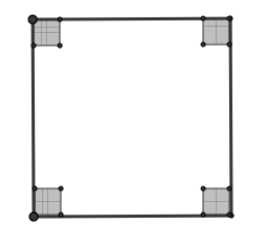
\includegraphics[scale=1]{hinhcau49}
\end{center}
\vspace{0.2cm}
\datcot
\bonpa
{\sai{$x=3a$.}}
{\sai{$x=2a$.}}
{\sai{$x=\dfrac{a}{2}$.}}
{\dung{$x=a$.}}
\end{question}

\begin{question}%%50
Một mặt cầu có thể tích $V$ đi qua đỉnh và đường tròn đáy của một hình nón có thiết diện qua trục là một tam giác đều. Tỷ số thể tích của phần khối cầu nằm ngoài khối nón và thể tích khối nón là
\vspace{0.2cm}
\datcot
\bonpa
{\sai{$\dfrac{9}{32}$.}}
{\dung{$\dfrac{23}{9}$.}}
{\sai{$\dfrac{32}{23}$.}}
{\sai{$\dfrac{32}{9}$.}}
\end{question}